%!TEX root = ../thesis.tex
%*******************************************************************************
%****************************** Third Chapter **********************************
%*******************************************************************************
\graphicspath{{Chapter3/Figs/Vector/}{Chapter3/Figs/}}

%%%%%%%%%%%%%%%%%%%%%%%%%%%%%%%%%%%%%%%%%%%%%%%%%%%%%%%%%%%%%%%%%%%%%%%%%%%%%%%%
% System Architecture
%%%%%%%%%%%%%%%%%%%%%%%%%%%%%%%%%%%%%%%%%%%%%%%%%%%%%%%%%%%%%%%%%%%%%%%%%%%%%%%%
% - What is most fitting solution to integrate TPS and UI into the
%   existing architecture?
%
\chapter{System Architecture}
\section{Introduction}
The term 'system' denotes "a set of things working together as parts of a mechanism or an interconnecting network". The family of systems that has formed through preceding architectural design decisions, must be able to integrate the new TPS system. Flows of information are to be aligned with adjacent system components so that dependencies are satisfied, while making use of the most fitting technologies for great adaptation. Existing conventions, methods and styles throughout the technical and conceptual spectrums are applied, enabling the system architecture to evolve consistently at one pace. Additionally, adjacent systems are improved by solutions introduced in this chapter.

%%%%%%%%%%%%%%%%%%%%%%%%%%%%%%%%%%%%%%%%%%%%%%%%%%%%%%%%%%%%%%%%%%%%%%%%%%%%%%%%
% Architectural Patterns
%%%%%%%%%%%%%%%%%%%%%%%%%%%%%%%%%%%%%%%%%%%%%%%%%%%%%%%%%%%%%%%%%%%%%%%%%%%%%%%%
% - Which architectural patterns fit in with the existing architecture?
%
\section{Architectural Patterns}
The current system architecture consists of three API's and nine services that connect to four databases, as can be seen in Figure \ref{fig:Architecture}. They provide functionalities to portals and mobile apps. The bigger and smaller shapes in the Figure represent large API's and smaller services respectively.

\begin{figure}[H]
	\centering
	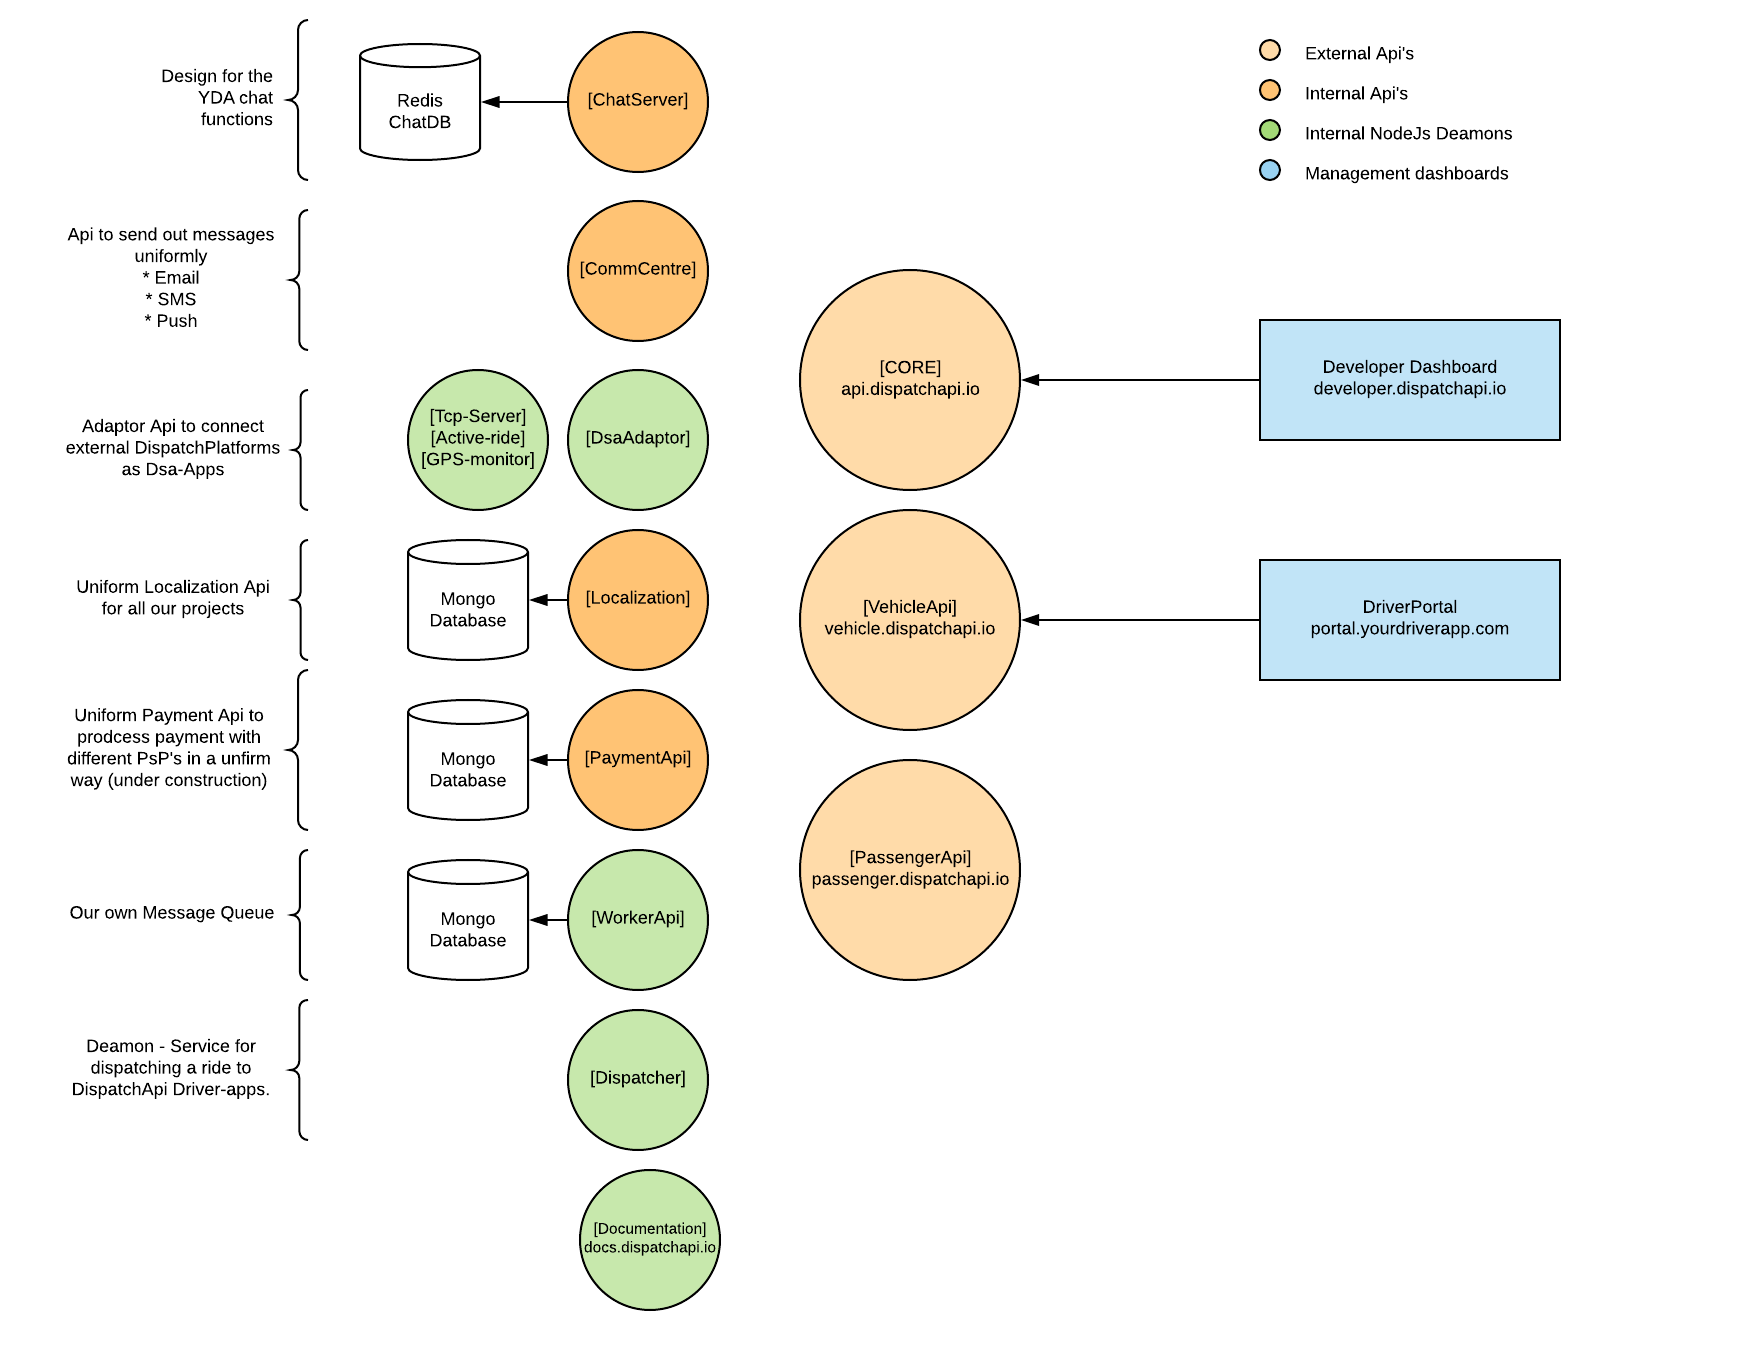
\includegraphics[width=1\textwidth]{Architecture}
	\caption[Current System Architecture]{Current System Architecture provided by taxiID.}
	\label{fig:Architecture}
\end{figure}

The orange colored services are used internally, the green shapes are used by external partners. The smaller services adhere to the pattern that is called service-oriented architecture, where application components provide services over a network typically. Within the architecture, a separation exists between user interfaces, business logic and data storage, that is known as the three-tier or multi-tier architecture, as described in \cite{IBM-3-tier}.

\subsection{Monoliths}
The bigger shapes in Figure \ref{fig:Architecture} may be classified as monoliths. In the context of computer software, a monolithic system may have different definitions. Rod Stephens captures the meaning of a monolithic architecture quite broadly: "In a monolithic architecture, a single program does everything. It displays the user interface, accesses data, processes customer offers, prints invoices, launches missiles, and does whatever else the application needs to do" in \cite{rod-BSE}. In general, a monolith describes a software application which is designed without modularity. Even though the frontend is separated in some cases, it fits the description most accurately. Integration of TPS could be achieved by implementing TPS as a component of a monolith. But what logically follows is either duplication, or dependencies between large systems. The first contradicts an important principle of software engineering; don't repeat yourself (DRY), the second limits scalability and independence of deployment. The legacy system has demonstrated this issue because it has its price calculation system implemented in this manner, now facing difficulties providing the price calculation functionality to newer projects.

\subsection{Microservices}
% https://resources.sei.cmu.edu/asset_files/Presentation/2016_017_001_454683.pdf

% \begin{figure}[H]
% 	\centering
% 	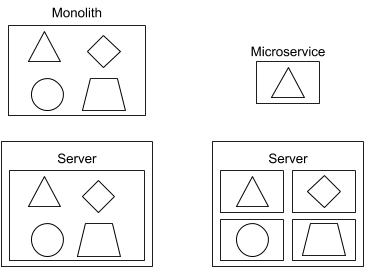
\includegraphics[width=0.6\textwidth]{MicroserviceMonolith}
% 	\caption[Monolith and Microservice]{Microservice and Monolith.}
% 	\label{fig:Microservice Monolith}
% \end{figure}

If the legacy price calculation system was implemented as a service, it could have been reused or replicated as a second separate price calculation system for YDA instead. A consensual definition of microservices does not exist, but can be defined as a development technique that structures a system architecture as multiple loosely coupled services, exactly opposing the description of a monolith. The smaller shapes in Figure \ref{fig:Architecture} can be described as miniservices or microservices. Philipp Hauer describes the advantages of independent services accurately in \cite{microservices}, mentioning; improvements in development speed through parallel development, isolated deployment and continuous delivery (CD), scalability and potential parallelism, and independence in case of failure. Fair points of criticism have been made in regard to microservices. Jan Stenberg has pointed out that microservices are information barriers in \cite{JS-microservices}, meaning that the process of implementing a new system is degraded by the sense of ownership of specific services by developers. Technical downsides that have been discussed in general are: latency, testing, deployment, security, and message formats.

\subsection{Frontend and Backend}
A model-view-controller pattern is separating the business and presentation layers in various frontend projects. This would mean that separate views have to be developed for each portal, or the views should be provided to the portals via iframes. In the last case, it may be beneficial to combine the frontend and backend in the same project structure. However, this would be in conflict with this three-tier pattern, which is not desired in respect to the evolution of the system architecture. Integration of the backend would mean that the core system should contain the price calculation system as a component, and separation of the backend would mean that the backend would be set up as a separate service. If this pattern is to be respected, four possibilities remain with which the frontend and backend could be implemented:

\begin{enumerate}
	\item Integrate views in existing portal, build TPS as a separate microservice
	\item Build separate service providing iframe views, build TPS as a separate microservice
	\item Integrate views in existing portal, integrate TPS as monolith component
	\item Build separate service providing iframe views, integrate TPS as monolith component
\end{enumerate}

The final decision, based on a comparison seen in table 4.1.1 in Appendix \ref{appendix:pregame}, proposes to separate the backend and integrate the frontend. This leaves the requirement of implementing the frontend in multiple portals simultaneously unresolved, but improves consistency of each individual portal implementation, and reduces dependencies of having to implement iframes.

%%%%%%%%%%%%%%%%%%%%%%%%%%%%%%%%%%%%%%%%%%%%%%%%%%%%%%%%%%%%%%%%%%%%%%%%%%%%%%%%
% Information Dependencies
%%%%%%%%%%%%%%%%%%%%%%%%%%%%%%%%%%%%%%%%%%%%%%%%%%%%%%%%%%%%%%%%%%%%%%%%%%%%%%%%
%
\section{Information Dependencies}
The frontend separation or integration cases have little influence on the further design of the system. The backend separation case however, is only possible if information dependencies are satisfied. User identifying information must be retrieved from a system containing the source of truth. Company and product information must be retrieved from adjecent systems, or stored in the trip pricing system database. Important data that must be acquired are: products, companies, applications, users, settings and VAT amounts. In isolation, this model contains all the required information to calculate a price, if the parameters shown in Listing \ref{lst:request} are provided.

\begin{center}
\noindent\begin{minipage}{.85\textwidth}
\begin{lstlisting}[caption={Minimal external information required for a trip price calculation.}, label={lst:request}]
	{
		"companyId": string
		"daAppInstallId": string,
		"vehicleTypes": string[],
		"passengerCount": number,
		"requestedDate": ISODate,
		"departure": { "gps": { "lat": string, "lng": string } },
		"destination": { "gps": { "lat": string, "lng": string } }
	}
\end{lstlisting}
\end{minipage}
\end{center}

The concrete data from the conceptual model could in theory be stored in one database, separate from the existing core database. How would the company data be synchronized? And does the system know which pricing rules should be used for the calculation? Assuming that companyId and daAppInstallId are provided in the authentication headers, the user can be identified. But this identity is futile if no pricing data is associated with it. There are three options with regard to storing the data in a way that user identity can be used to associate pricing information:

\begin{enumerate}
	\item Centralized state - A single centralized database
	\item Distributed state - Multiple distributed synchronized databases
	\item Minimal state - Multiple independent databases with stateless references
\end{enumerate}

A single source of truth, central database, would avoid having duplicate data all together. No synchronization, thus no network communication is necessary, and all data is always readily available. This design desecrates the independence aspect of microservices. The multiple synchronized databases in option 2, raises the problem of having duplicate, out of sync data. A one-way dataflow could reduce this problem, but it is not always entirely avoidable. This design does adhere to the concept of microservices by allowing independent deployments still. The minimal state option 3, would improve on the previous option 2, by only allowing data to be referenced back in a stateless manner. This means that a company in the core database could have related data stored in the TPS database, without being 'aware' of it. The entities that reference the company can be used in an autonomous fashion, where only the necessary information is sent to TPS whenever a request is made. Multiple proposal were made aiming to solve the combination of authentication, authorization and data consistency problems.

%%%%%%%%%%%%%%%%%%%%%%%%%%%%%%%%%%%%%%%%%%%%%%%%%%%%%%%%%%%%%%%%%%%%%%%%%%%%%%%%
% Authentication and Authorization
%%%%%%%%%%%%%%%%%%%%%%%%%%%%%%%%%%%%%%%%%%%%%%%%%%%%%%%%%%%%%%%%%%%%%%%%%%%%%%%%
% - How can authentication between services be implemented or improved?
%
\section{Authentication and Authorization}
In the legacy system, authorization was achieved by sending extra headers for each crucial piece of information, this is clarified in Appendix \ref{appendix:pregame}, chapter 3.4. To prevent data duplication, the microservice could be connected to the database that is used by the core system. But this makes the microservice less decoupled, and directly contradicts the desire to separate data dependencies. In the slides of Appendix \ref{appendix:slides_2_authentication} four examples options are listed as to which authentication could be implemented. These examples are based on three proposals listed in Appendix \ref{appendix:pregame}, chapter 4.4, which are further explained in the subsections below.

\subsection{OAuth 2.0}
This authentication mechanism delegates user identity management to a separate authentication service that, similar to the pricing microservice, has its own single task of authenticating users. OAuth 2.0 is a protocol that has been designed to allow third-party apps to grant access to an HTTP service on behalf of the resource owner. Although granting permissions should not necessarily be done by any user, this mechanism could be used for authentication purposes in the way that Facebook login would work as a central verification authority. The token is verified by the authority authentication server on each request, keeping the user identity management centralized inside one single service.

\begin{figure}[H]
	\centering
	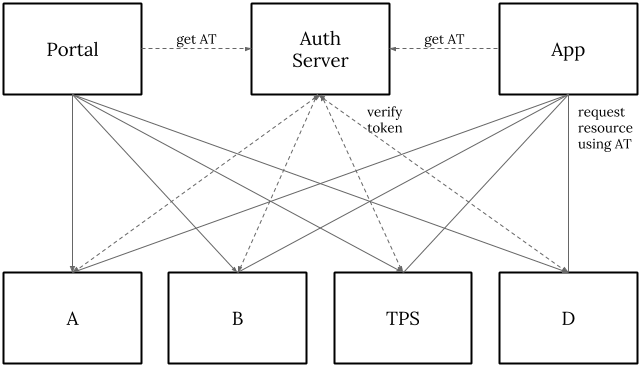
\includegraphics[width=.7\textwidth]{Auth1}
	\caption[Proposal OAuth 2.0]{OAuth requests where tokens are verified by Auth Server.}
	\label{fig:Auth1}
\end{figure}

This proposal is used in example four of Appendix \ref{appendix:slides_2_authentication}.

\subsection{JSON Web Token}
This proposal entirely removes the database connection to any user data. This is possible when a JSON Web Token (JWT) is used. A JWT may be signed with a cryptographic algorithm or even a public/private key pair using RSA. After the user enters valid credentials, the core system validates the credentials by comparing them with user data in the database.

\begin{center}
\noindent\begin{minipage}{.85\textwidth}
\begin{lstlisting}[caption={Two user identifiers and registered claim names stored inside the payload of a JSON web token.}, label={lst:payload}]
	{
		"companyId": "59ea0846f1fea03858e16311",
		"daAppInstallId": "599d39b67c4cae5f11475e93",
		"iat": 1521729818,
		"exp": 1521816218,
		"aud": "tps.dispatchapi.io",
		"iss": "api.dispatchapi.io",
		"sub": "getPrices"
	}
\end{lstlisting}
\end{minipage}
\end{center}

The keys other than companyId and daAppInstallId describe expiration date of the token, and other meta information. The core system signs a token that with a secret that is known by the microservice. The token consists of three parts, separated by a full stop. The first part (header) of the token contains information about the hashing algorithm that is used to encrypt the payload. This part is Base64Url encoded. The payload itself contains information stored in JSON format as shown in Listing \ref{lst:payload}. The identity of the user is stored in the payload that can only be revealed by whoever holds the secret with which it is signed. Then the message can be verified using the third part of the token, which is the signature. The verification step prevents tampering with the payload. Claims can be added to the payload as shown in \ref{lst:payload} to provide information about the token, as explained in \cite{JWT}. Figure \ref{fig:Auth2} adds statelessness to the previous proposal, thereby removing the verification step with the authentication server.

\begin{figure}[H]
	\centering
	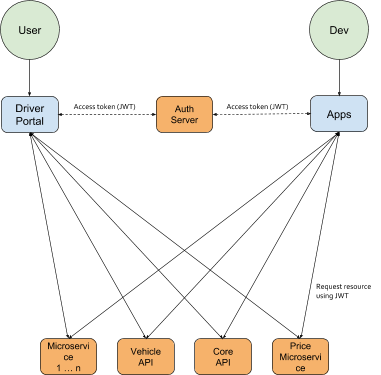
\includegraphics[width=.7\textwidth]{Auth2}
	\caption[Proposal Stateless JWT]{OAuth with stateless JWT requests.}
	\label{fig:Auth2}
\end{figure}

\subsection{API Gateway}
The final proposal allows services to be used by external agents via the API Gateway. This solution allows for a central middleware in which authentication and authorization is handled, where the microservices are shielded from public access, and all communication is established through the API Gateway \cite{api-gateway}. Next to authentication, the gateway could optimize the endpoints so that no multiple requests are needed from external agents to gather different types of resources. These calls could be made internally to the microservices behind the gateway. This also opens the possibility the freely change the microservices without changing the public endpoints exposed by the gateway, and even offers slow or instant transitions to different versions of microservices. The different proposals explain the improvements they may bring over some system. But the advice given is not tied to this project, instead to the entire Dispatch API. It’s advised to have a constructive dialogue about the future of the company, and the way it’s planning to scale. One could put a API Gateway in front of a monolithic app to help with transitioning to a microservice-oriented app.

\begin{figure}[H]
	\centering
	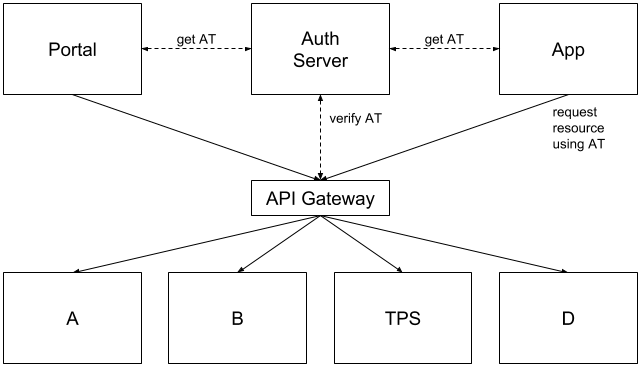
\includegraphics[width=.7\textwidth]{Auth3}
	\caption[Proposal API Gateway]{API Gateway.}
	\label{fig:Auth3}
\end{figure}

The fourth example is proposed as the best possible solution as shown in Appendix \ref{appendix:slides_2_authentication}. This solution would use the single responsibility authentication service as shown in Figure \ref{fig:Auth1}, and the minimal state option as shown in Figure \ref{fig:Auth2}. A successful login would yield a JWT from a dedicated authentication service. A database with a single source of truth would allow the authentication service to provide truthful user identifying information. The JWT would allow every system to acquire user identifying information from the token payload, and keep from having token verification round-trips. The only synchronization steps are executed when a new company or application is created, or when they are deleted. The proposal completely decouples the information requirements by keeping Core data and TPS data in their respective databases separated.

%%%%%%%%%%%%%%%%%%%%%%%%%%%%%%%%%%%%%%%%%%%%%%%%%%%%%%%%%%%%%%%%%%%%%%%%%%%%%%%%
% Methods and Techniques
%%%%%%%%%%%%%%%%%%%%%%%%%%%%%%%%%%%%%%%%%%%%%%%%%%%%%%%%%%%%%%%%%%%%%%%%%%%%%%%%
%
\section{Methods and Techniques}
All API projects in taxiID have been developed using JavaScript, with the exception of one legacy PHP project. Java and Swift are used for mobile applications. It is not beneficial to explore every single possible combination of technologies, as the range of possibilities is too big. But it is important to look at some popular alternatives. NodeJS offers more modern features and abilities to separate concerns in comparison with PHP. Speed and consistency of the codebase are important reasons to opt for a JavaScript NodeJS project, as advised in Appendix \ref{appendix:pregame}, chapter 4.6. Two proofs of concept were made, one showcasing an Express solution using GraphQL to expose resource, and the other exposing resources using Loopback in a hybrid JavaScript Typescript project.

\subsection{Backend Framework}
The first proof of concept allows consumers of the API to dictate the information that they want to receive. Using this concept, an API Gateway could easily chain requests, mapping resources from multiple services to a single endpoint. The proof of concept is available at \url{github.com/Menziess/Typescript-GraphQL-API}. This proof of concept was not advised to be used for TPS, because the inconsistencies between services introduce unnecessary complexity for developers. The first solution is vastly different from existing projects, which will introduce inconsistencies once again. For example, one API could make network requests to separate Loopback API's, but then has to implement a new inconsistent request format to deal with a GraphQL API. And this activity is repeated for all other depending API's and applications. For this reason, the second proof of concept has been chosen to start the project with. The team has experience with LoopBack 3.0 \cite{lb}, enabling the team to reuse code, maintain their development velocity, and reason about this project more effectively. The project structure as shown in Appendix \ref{appendix:slides_2} is made up of of Loopback configuration files, and Typescript files containing important logic. This separation is not ideal, but expresses the fact that some JavaScript files belong to a framework, and must adhere to a special framework format. The Typescript files offer more strict checks through static typing, interfaces and classes.

\subsection{Frontend Framework}
The first non-functional requirement states that the solution should be seamlessly integrated in the portal. On top of that, a user shouldn’t have to log in again to make use of the pricing service from within that portal. For the portal, a proof of concept was made for the case of having the portal implemented as a separate project. The proof of concept is available at \url{github.com/Menziess/Typescript-Reiskosten}. This concept was used to illustrate the differences between Vue and Angular, embodying mostly application structure. Angular being more suitable for large corporate application, while Vue caters toward smaller, more flexible, less structured applications. Iframes, objects and embeds have been mentioned as potential solutions to integrate a frontend in several distinct portals. This problem affects more than just the pricing project, therefore a decision must be made on a higher level before the frontend will be integrated, but the decision is not required for the first sprint to start. The YourDriverApp portal has been constructed using Angular 5. If the frontend is to be integrated, Angular will be the framework that is used to construct the views.

\subsection{Database}
Agarwal and Rajan state that NoSQL takes advantage of cheap memory and processing power, thereby handling the four V’s of big data more effectively, but lacks robustness in comparison to SQL databases in \cite{AGS}. Performance of geoWithin and geoIntersect queries have been tested between PostGIS and MongoDB. The report dives deeper into spatial queries and concludes that their tests suggest that MongoDB performs better by an average factor of 10, which increases exponentially as the data size increases, but lacks spatial functions that OpenGIS supports. Indexing of spatial fields is said to have a big impact on performance. The conclusion states that the downside of using NoSQL compared to SQL is the limitation in respect to spatial functions. The previous chapter discussed important features that were required for the location matching functionality to operate properly. Both OGC and GeoJSON standards offered sufficient support. In the paper of Schmid et al. 2015 \cite{SCS}, the team argues that clustering is much easier in MongoDB, which may be important in the future when a company grows. In respect to the CAP theorem, and ACID properties, SQL and MySQL have different strengths and weaknesses:

\begin{table}[htbp!]
	\centering
	\begin{tabular}{c|c|c}
		\toprule
		& SQL & NoSQL \\
		\midrule
		Integrity & \checkmark\checkmark & x \\
		Scaling & x & \checkmark\checkmark \\
		Atomicity & \checkmark & \checkmark \\
		Consistency & \checkmark\checkmark & \checkmark \\
		Isolation & \checkmark & \checkmark \\
		Durability & \checkmark & \checkmark \\
		Availability & \checkmark & \checkmark\checkmark \\
		Partition Tolerance & \checkmark & \checkmark \\
		Performance & \checkmark & \checkmark\checkmark \\
		Maturity & \checkmark\checkmark & \checkmark \\
		JSON Documents & x & \checkmark \\
		Clustering & \checkmark & \checkmark \\
		Sharding & \checkmark & \checkmark\checkmark \\
		\bottomrule
	\end{tabular}
	\caption[Databases Comparison]{Comparison between SQL and NoSQL databases.}
	\label{tab:databases-comparison}
\end{table}

Performance and scalability are important properties for taxiID's systems. MongoDB has the ability to scale horizontally. Because MongoDB has good sharding capabilities, location related performance issues may be solved by setting up local database systems. NoSQL document storage allows for great horizontal scaling and sharding, catering more towards use cases that do not require overall consistency of the data, but makes the data highly available. Performance of spatial queries is very important, for which the conclusion of Agarwal and Rajan support the use of NoSQL.

%%%%%%%%%%%%%%%%%%%%%%%%%%%%%%%%%%%%%%%%%%%%%%%%%%%%%%%%%%%%%%%%%%%%%%%%%%%%%%%%
% Premise
%%%%%%%%%%%%%%%%%%%%%%%%%%%%%%%%%%%%%%%%%%%%%%%%%%%%%%%%%%%%%%%%%%%%%%%%%%%%%%%%
%
\section{Conclusion on System Architecture}
\[\textit{What is most fitting solution to integrate the backend and frontend into the existing architecture?}\] \hfill

A NodeJS loopback microservice should be implemented along with a MongoDB database, resulting in a scalable high performance solution that can be deployed independently. Introducing a stateless authentication service to implement identity management, allowing the microservice to be more decoupled, bringing the amount of verification requests down to zero. This solution is most fitting to the existing architecture, that only has to implement one future proof authentication method.
